\documentclass{beamer}
\usetheme{Montpellier}
%\usecolortheme{rose}
\useinnertheme{rounded}
\setbeamersize{text margin left=5mm,text margin right=10mm}
\usefonttheme{serif}
\usepackage{graphicx}
\usepackage[italian]{babel}
\usepackage[utf8]{inputenc}
\usepackage{tabularx}
\usepackage{tikz}
\usepackage[absolute,overlay]{textpos} 
\usepackage{xcolor}
\usepackage{multicol}
\definecolor{myGreen}{RGB}{54, 114, 89}
\definecolor{unipd}{RGB}{155, 0, 20}
% Per il tema Montpellier
\setbeamercolor{separation line}{bg=myGreen!20}
\setbeamercolor{title in head/foot}{bg=white, fg=myGreen}
\setbeamercolor{section in head/foot}{bg=white, fg=myGreen}
\setbeamercolor{subsection in head/foot}{bg=white, fg=myGreen}
\setbeamercolor{background canvas}{bg=white}
\setbeamercolor{title}{fg=unipd}
\setbeamercolor{item}{fg =myGreen}
\setbeamercolor{frametitle}{fg = myGreen}
\setbeamercolor{section in toc}{fg=myGreen!80}
\setbeamercolor{subsection in toc}{fg=black}
\setbeamerfont{section in toc}{series=\bfseries,size=\normalsize}
\setbeamerfont{frametitle}{series=\bfseries}
%\setbeamerfont{title}{family=\scshape}
%\setbeamercolor{frametitle}{fg=unipd}
%\setbeamercolor{section in head/foot}{bg=unipd, fg=white}
%\setbeamercolor{subsection in head/foot}{fg=unipd}
%\setbeamercolor{author in head/foot}{bg=unipd, fg=white}
%\setbeamercolor{title in head/foot}{fg=unipd}
%\setbeamercolor{date in head/foot}{fg=unipd}

% definisce gli elementi da mettere sopra la figura 
% rectangles on figures 
\newcommand{\imagenode}[2][1]% [scale], filename
{   \node[above right,inner sep=0] (myimage) {\includegraphics[scale=#1]{#2}};
	\path (myimage.north east);
	\pgfgetlastxy{\myimagex}{\myimagey}
	\pgfmathsetmacro{\myimagewidth}{\myimagex/28.453}
	\pgfmathsetmacro{\myimageheight}{\myimagey/28.453}
}
\newcommand{\imagegrid}[4][help lines]% [options], steps, font, precision
{   \pgfkeys{/pgf/number format/.cd,fixed,precision=#4}
	\foreach \x in {0,...,#2}
	{   \draw[#1] (\x/#2*\myimagewidth,\myimageheight) -- (\x/#2*\myimagewidth,0) node[below] {#3\pgfmathparse{\x/#2}\pgfmathprintnumber{\pgfmathresult}};
		\draw[#1] (\myimagewidth,\x/#2*\myimageheight) -- (0,\x/#2*\myimageheight) node[left] {#3\pgfmathparse{\x/#2}\pgfmathprintnumber{\pgfmathresult}};
	}
}

\newcommand{\highlightbox}[8][densely dashed,thick]% [options], left, low, right, up, node options, node text, overlay spec
{   \only<#8>{\draw[#1] (#2*\myimagewidth, #3*\myimageheight) rectangle node[#6] {#7} (#4*\myimagewidth, #5*\myimageheight);}
}

\newcommand{\highlighttext}[8][densely dashed,thick]% [options], left, low, right, up, node options, node text, overlay spec
{   \only<#8>{\path[#1] (#2*\myimagewidth, #3*\myimageheight) rectangle node[#6] {#7} (#4*\myimagewidth, #5*\myimageheight);}
}

% tikz per la cfa 

\usetikzlibrary{shapes.geometric, arrows}
\tikzstyle{latent} = [ellipse, minimum width=2.5cm, minimum height=2cm,text centered, draw=black]
\tikzstyle{item} = [rectangle, rounded corners, minimum width=0.5cm, minimum height=1cm, text width =1.5cm, text centered, draw=black]
\tikzstyle{arrow} = [thick,->,>=stealth]

\AtBeginSection[]
{
	\begin{frame}
		\tableofcontents[currentsection, currentsubsection]
	\end{frame}
}

\AtBeginSubsection[]
{
	\begin{frame}
		\tableofcontents[currentsection, currentsubsection]
	\end{frame}
}


\title[Meaningfullness]{Le misure in psicologia sono significanti?\\ Il caso del test della Torre di Londra.}
\author[Epifania et al.]{\textbf{Ottavia M. Epifania}, Luca Stefanutti, Pasquale Anselmi,  Andrea Brancaccio, Debora de Chiusole}
\institute [UniPd] {
	
\includegraphics[width=10mm]{unipd.png}\\ 
Dipartimento di Filosofia, Sociologia, Pedagogia e Psicologia Applicata,\\	Università di Padova}
	
	\date [AIP2023] {%\vspace{0.6cm}\\
		Convegno AIP-Sezione Sperimentale 2023\\ Simposio: Crisi di replicabilità o crisi di validità? L’importanza delle misure \\ \vspace{3mm}
		19 Settembre 2023}
\begin{document}
	
	\begin{frame}[plain]
		\maketitle
	\end{frame}

\section{La significanza}

\begin{frame}
	
	
\end{frame}

\section{Il caso}
\subsection{La Torre di Londra}
\begin{frame}
	
	L'obietivo della Torre di Londra (ToL) è di raggiungere lo \emph{stato obiettivo} da uno \emph{stato iniziale} nel minimo numero di mosse.\\
	\vspace{.1cm}
	\vspace{.2cm}
	\begin{columns}
		\column{0.45\textwidth}
		\begin{center}
			\begin{tikzpicture}[scale=1.2]
				\node[mark=diamond,inner sep = 0pt, minimum size = 4pt] (23) at (  -1.5,  3.5*1.73) {
					\begin{tikzpicture}[scale=.6]
						\draw[draw=black!20,fill=black!20] (0,5) rectangle (6,5.3);
						\draw[draw=black!20,fill=black!20] (0.85,5) rectangle (1.15,8.5);
						\draw[draw=black!20,fill=black!20] (2.85,5) rectangle (3.15,7.5);
						\draw[draw=black!20,fill=black!20] (4.85,5) rectangle (5.15,6.5);
						\draw[fill=red] (1,5.8) circle (15pt);
						\draw[fill=yellow] (5,5.8) circle (15pt);
						\draw[fill= blue] (3,5.8) circle (15pt);
					\end{tikzpicture}
				};
			\end{tikzpicture}\\
			Stato iniziale
		\end{center}
		\column{0.45\textwidth}
		\begin{center}
			\begin{tikzpicture}[scale=1.2]
				\node[mark=diamond,inner sep = 0pt, minimum size = 4pt] (23) at (  -1.5,  3.5*1.73) {
					\begin{tikzpicture}[scale=.6]
						\draw[draw=black!20,fill=black!20] (0,5) rectangle (6,5.3);
						\draw[draw=black!20,fill=black!20] (0.85,5) rectangle (1.15,8.5);
						\draw[draw=black!20,fill=black!20] (2.85,5) rectangle (3.15,7.5);
						\draw[draw=black!20,fill=black!20] (4.85,5) rectangle (5.15,6.5);
						\draw[fill=yellow] (1,5.8) circle (15pt);
						\draw[fill=red] (1,6.85) circle (15pt);
						\draw[fill=blue] (3,5.8) circle (15pt);
					\end{tikzpicture}
				};
			\end{tikzpicture}\\
			Stato obiettivo
		\end{center}
	\end{columns}
	
\end{frame}

\begin{frame}{Caratteristiche delle Torre di Londra}{Kaller, Unterrainer, Rahm, \& Halsband (2004)}
	Le caratteristiche strutturali che influenzano le performance di pianificazione hai problem della TOL sono:\\
	\vspace{.3cm}
	\begin{itemize}
		\item Il numero di mosse minimo per risolvere il problema\\
		\vspace{.2cm}
		\item Il numero di soluzioni alternative \\
		\vspace{.2cm}
		\item La gerarchia dello stato iniziale e/o finale\\
	\end{itemize}
	\vspace{.2cm}
	\hspace{.5cm}
	\begin{tikzpicture}[scale=1.2]
		\node[mark=diamond,inner sep = 0pt, minimum size = 4pt] (23) at (  -1.5,  3.5*1.73) {
			\begin{tikzpicture}[scale=.4]
				\draw[draw=black!20,fill=black!20] (0,5) rectangle (6,5.3);
				\draw[draw=black!20,fill=black!20] (0.85,5) rectangle (1.15,8.5);
				\draw[draw=black!20,fill=black!20] (2.85,5) rectangle (3.15,7.5);
				\draw[draw=black!20,fill=black!20] (4.85,5) rectangle (5.15,6.5);
				\draw[fill=yellow] (1,5.8) circle (15pt);
				\draw[fill=red] (1,6.85) circle (15pt);
				\draw[fill=blue] (3,5.8) circle (15pt);
			\end{tikzpicture}
		};
		
		\node[mark=diamond,inner sep = 0pt, minimum size = 4pt] (23) at (  2,  3.5*1.73) {
			\begin{tikzpicture}[scale=.4]
				\draw[draw=black!20,fill=black!20] (0,5) rectangle (6,5.3);
				\draw[draw=black!20,fill=black!20] (0.85,5) rectangle (1.15,8.5);
				\draw[draw=black!20,fill=black!20] (2.85,5) rectangle (3.15,7.5);
				\draw[draw=black!20,fill=black!20] (4.85,5) rectangle (5.15,6.5);
				\draw[fill=yellow] (1,5.8) circle (15pt);
				\draw[fill=red] (5,5.8) circle (15pt);
				\draw[fill=blue] (3,5.8) circle (15pt);
			\end{tikzpicture}
		};
		
		\node[mark=diamond,inner sep = 0pt, minimum size = 4pt] (23) at (  5.5,  3.5*1.73) {
			\begin{tikzpicture}[scale=.4]
				\draw[draw=black!20,fill=black!20] (0,5) rectangle (6,5.3);
				\draw[draw=black!20,fill=black!20] (0.85,5) rectangle (1.15,8.5);
				\draw[draw=black!20,fill=black!20] (2.85,5) rectangle (3.15,7.5);
				\draw[draw=black!20,fill=black!20] (4.85,5) rectangle (5.15,6.5);
				\draw[fill=yellow] (1,5.8) circle (15pt);
				\draw[fill=red] (1,6.85) circle (15pt);
				\draw[fill=blue] (1,7.9) circle (15pt);
			\end{tikzpicture}
		};
		
	\end{tikzpicture}
\end{frame}


\begin{frame}{Il Test della Torre di Londra (ToL test)}{Shallice (1982)}
	\begin{columns}
		\column{0.45\textwidth}
		
		\begin{center}
			\small
			\begin{itemize}
				\item Nello spazio problema della ToL è possibile definire $36\times 35=1260$ problemi
				\vspace{.2cm}   
				\item Shallice nel 1982 ha scelto 12 problemi   
				\vspace{.2cm}
				\item Il ToL test ha lo stato iniziale fissato e gli stati obiettivo che variano 
			\end{itemize}
			
			\vspace{.3cm}
			\begin{tikzpicture}[scale=1.2]
				\node[mark=diamond,inner sep = 0pt, minimum size = 4pt] (23) at (  -1.5,  3.5*1.73) {
					\begin{tikzpicture}[scale=.4]
						\draw[draw=black!20,fill=black!20] (0,5) rectangle (6,5.3);
						\draw[draw=black!20,fill=black!20] (0.85,5) rectangle (1.15,8.5);
						\draw[draw=black!20,fill=black!20] (2.85,5) rectangle (3.15,7.5);
						\draw[draw=black!20,fill=black!20] (4.85,5) rectangle (5.15,6.5);
						\draw[fill=yellow] (1,5.8) circle (15pt);
						\draw[fill=red] (1,6.85) circle (15pt);
						\draw[fill=blue] (3,5.8) circle (15pt);
					\end{tikzpicture}
				};
			\end{tikzpicture}
		\end{center}
		
		\column{0.45\textwidth}
		\vspace{- .5cm}
		\begin{center}    
			\scriptsize
			I dodici problemi di Shallice \\
			
			\vspace{ .2cm}
			\begin{tabular}{ccc}
				\hline
				Problemi	&	N di mosse	&	N di percorsi	\\
				\hline
				Esempio	&	2	&	1	\\
				1	&	2	&	1	\\
				2	&	2	&	1	\\
				3	&	3	&	2	\\
				4	&	3	&	1	\\
				5	&	4	&	2	\\
				6	&	4	&	1	\\
				7	&	4	&	1	\\
				8	&	4	&	1	\\
				9	&	5	&	2	\\
				10	&	5	&	1	\\
				11	&	5	&	1	\\
				12	&	5	&	2	\\
				\hline
			\end{tabular}
		\end{center}
	\end{columns}
\end{frame}

\subsection{I metodi di scoring}

\begin{frame}

		\begin{alertblock}{Shallice scoring 1 (SH1)}
\small{
	\begin{tabular}{c c c c}
	\hline
	\multicolumn{2}{c}{Tempi di risposta} & \multicolumn{2}{c}{Accuratezze} \\
	\hline
	Scoring & Se \emph{tr} & Scoring & Se \\\hline
	1 & $< 60$ \emph{s} & 1 & Corretto al primo tentativo \\
	0 & $> 60$ \emph{s} & 0 & Più di un tentativo \\ \hline
\end{tabular}
}
					
			
			Punteggio di ogni item: $0$ -- $1$
			
			Punteggio massimo: 12

		
		
			
					\end{alertblock}
		
				\begin{exampleblock}{Shallice scoring 2}
		\scriptsize
		
\begin{tabular}{c c}
	\hline
	Scoring & Tempo di risposta \\ \hline
	3 & $< 15$ \emph{s} \\
	2 & $< 30$ \emph{s} \\
	1 & $< 60$ \emph{s} \\
	0 & $< 60$ \emph{s} \\
	\hline
\end{tabular}
				\end{exampleblock}
		

				\begin{exampleblock}{AN}
			
		\end{exampleblock}
		
		\begin{alertblock}{KR}
			
		\end{alertblock}


\end{frame}

\section{Lo studio}
	
	\begin{frame}{Il campione}
		
		\begin{itemize}
			\item Dettagli sulla composizione del campione (genere per fasce di età che ho definito)
			
			\item Dettagli sulla loro performance ``grezza'' su accuratezze e tempi per maschi e femmine $\rightarrow$ In realtà non è così semplice. Considero solo il primo tentativo? Considero il tempo della somma dei tre tentativi? come considero la rispsita corretta? Io sarei per: 
			
			\begin{itemize}
				\item Considero solo il tempo al primo tentativo
				\item Considero l'item corretto solo se risolto al primo tentativo
			\end{itemize}
			
		\end{itemize}
		
			\end{frame}


\begin{frame}{Le correlazioni}
	
	\begin{figure}
		\centering
		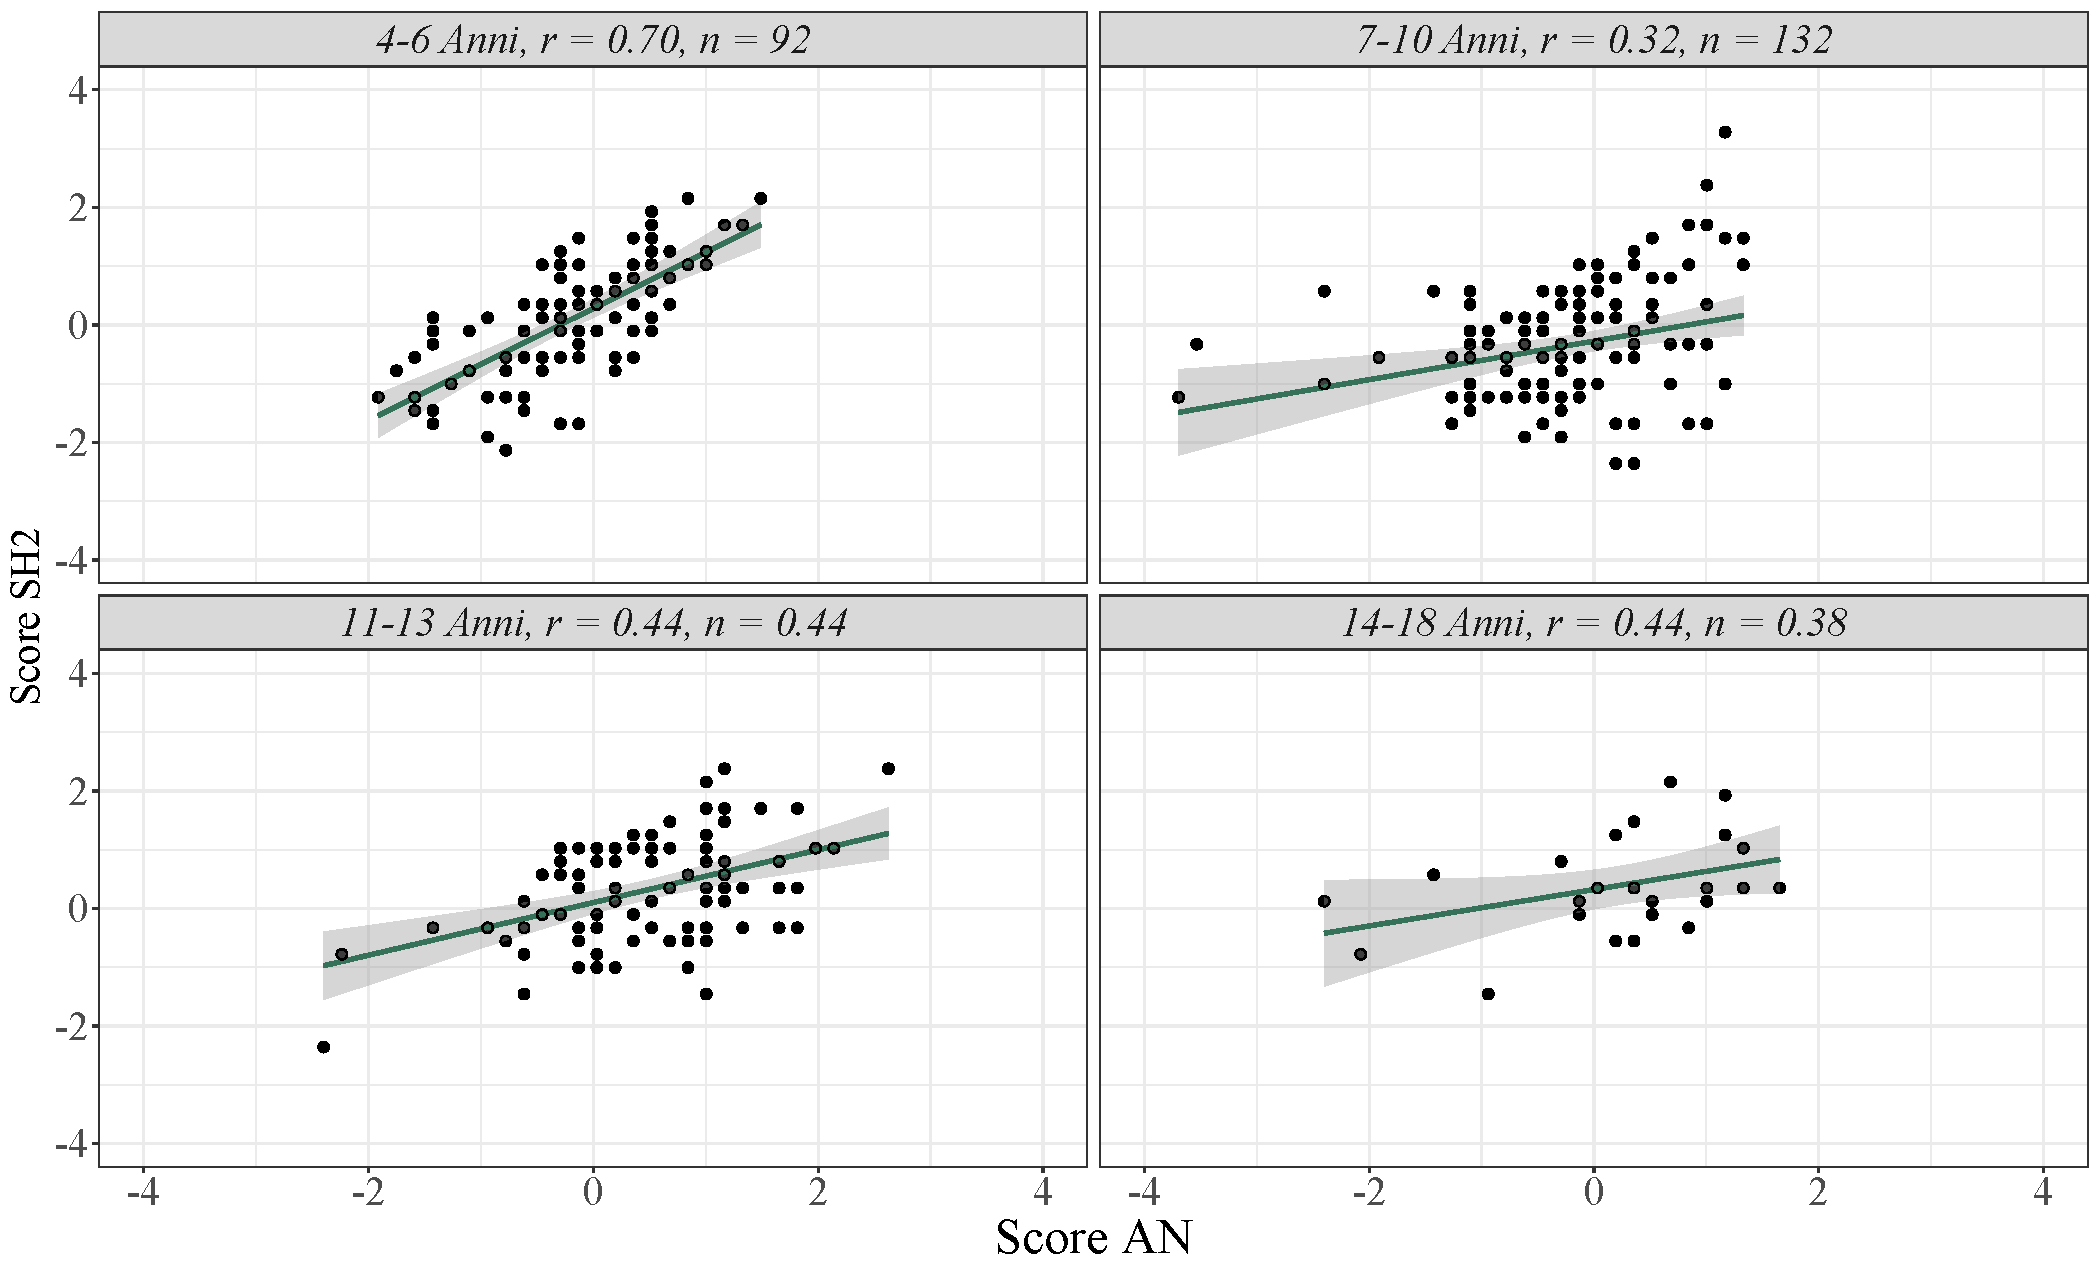
\includegraphics[width=\linewidth]{img/correlazioni_gruppi.pdf}
	\end{figure}
	
\end{frame}


\begin{frame}{Quanto è realmente grave?}
	

		
Ogni soggetto viene confrontato contro tutti gli altri: 

\vspace{3mm}

\begin{itemize}
\item  Confronto SH2 ($\Delta_{\text{SH2}}$): calcolata la differenza tra i punteggi standardizzati di SH2 tra coppie di soggetti 

\item  Confronto AN ($\Delta_{\text{AN}}$): calcolata la differenza tra i punteggi standardizzati di AN tra coppie di soggetti (ogni soggetto confrontato con tutti gli altri)
\end{itemize}


\begin{center}
	$\Delta_{\text{SH2}}$ vs. $\Delta_{\text{AN}}$
\end{center}


\end{frame}


\begin{frame}
	\begin{overprint}
		
		\onslide<1>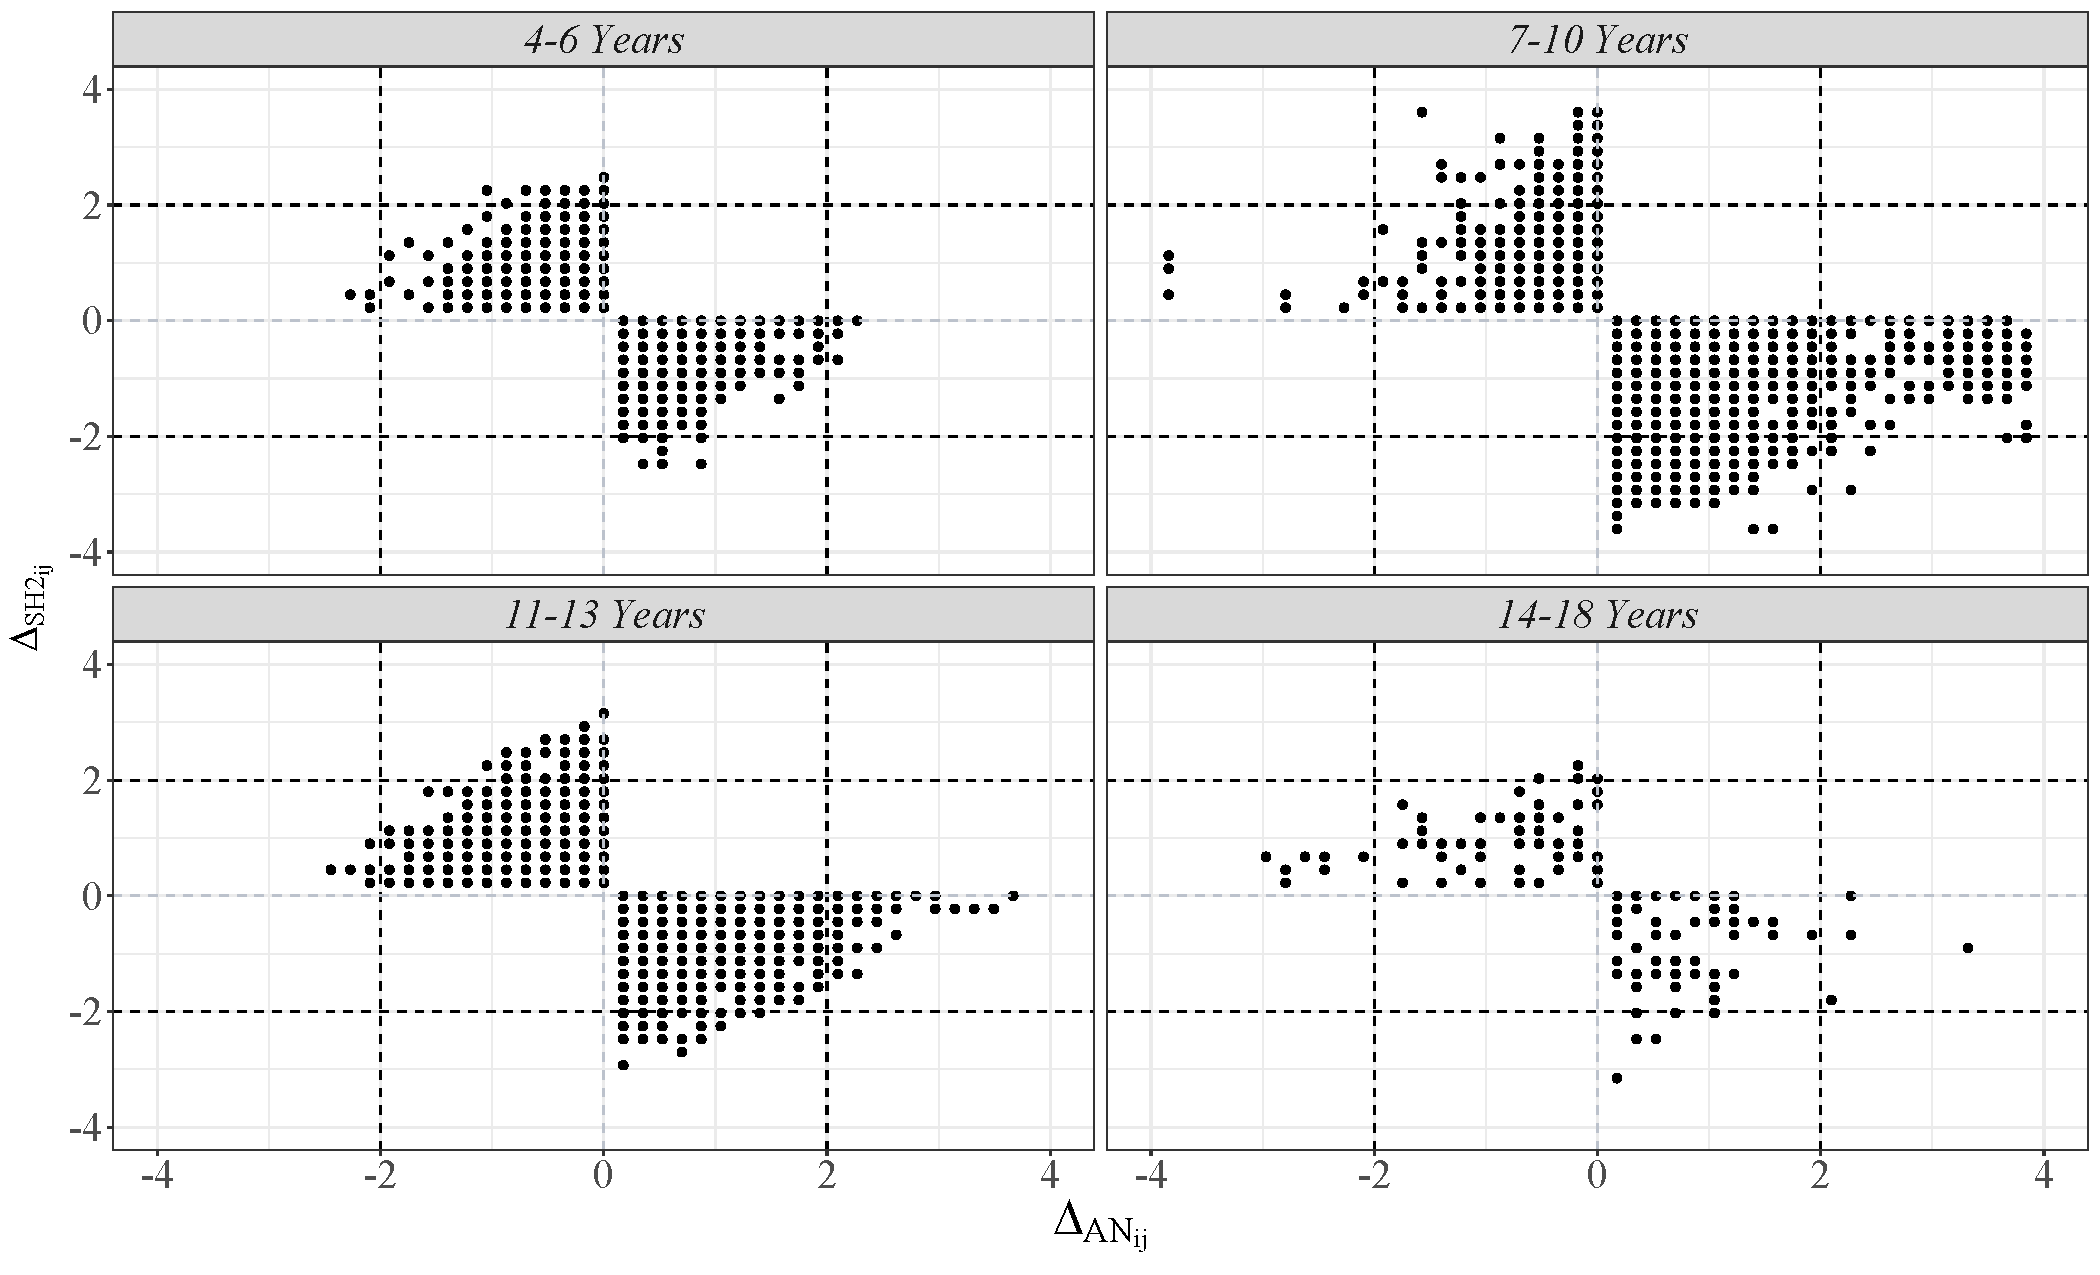
\includegraphics[width=\linewidth]{img/farfalle_gruppi.pdf}
		\onslide<2>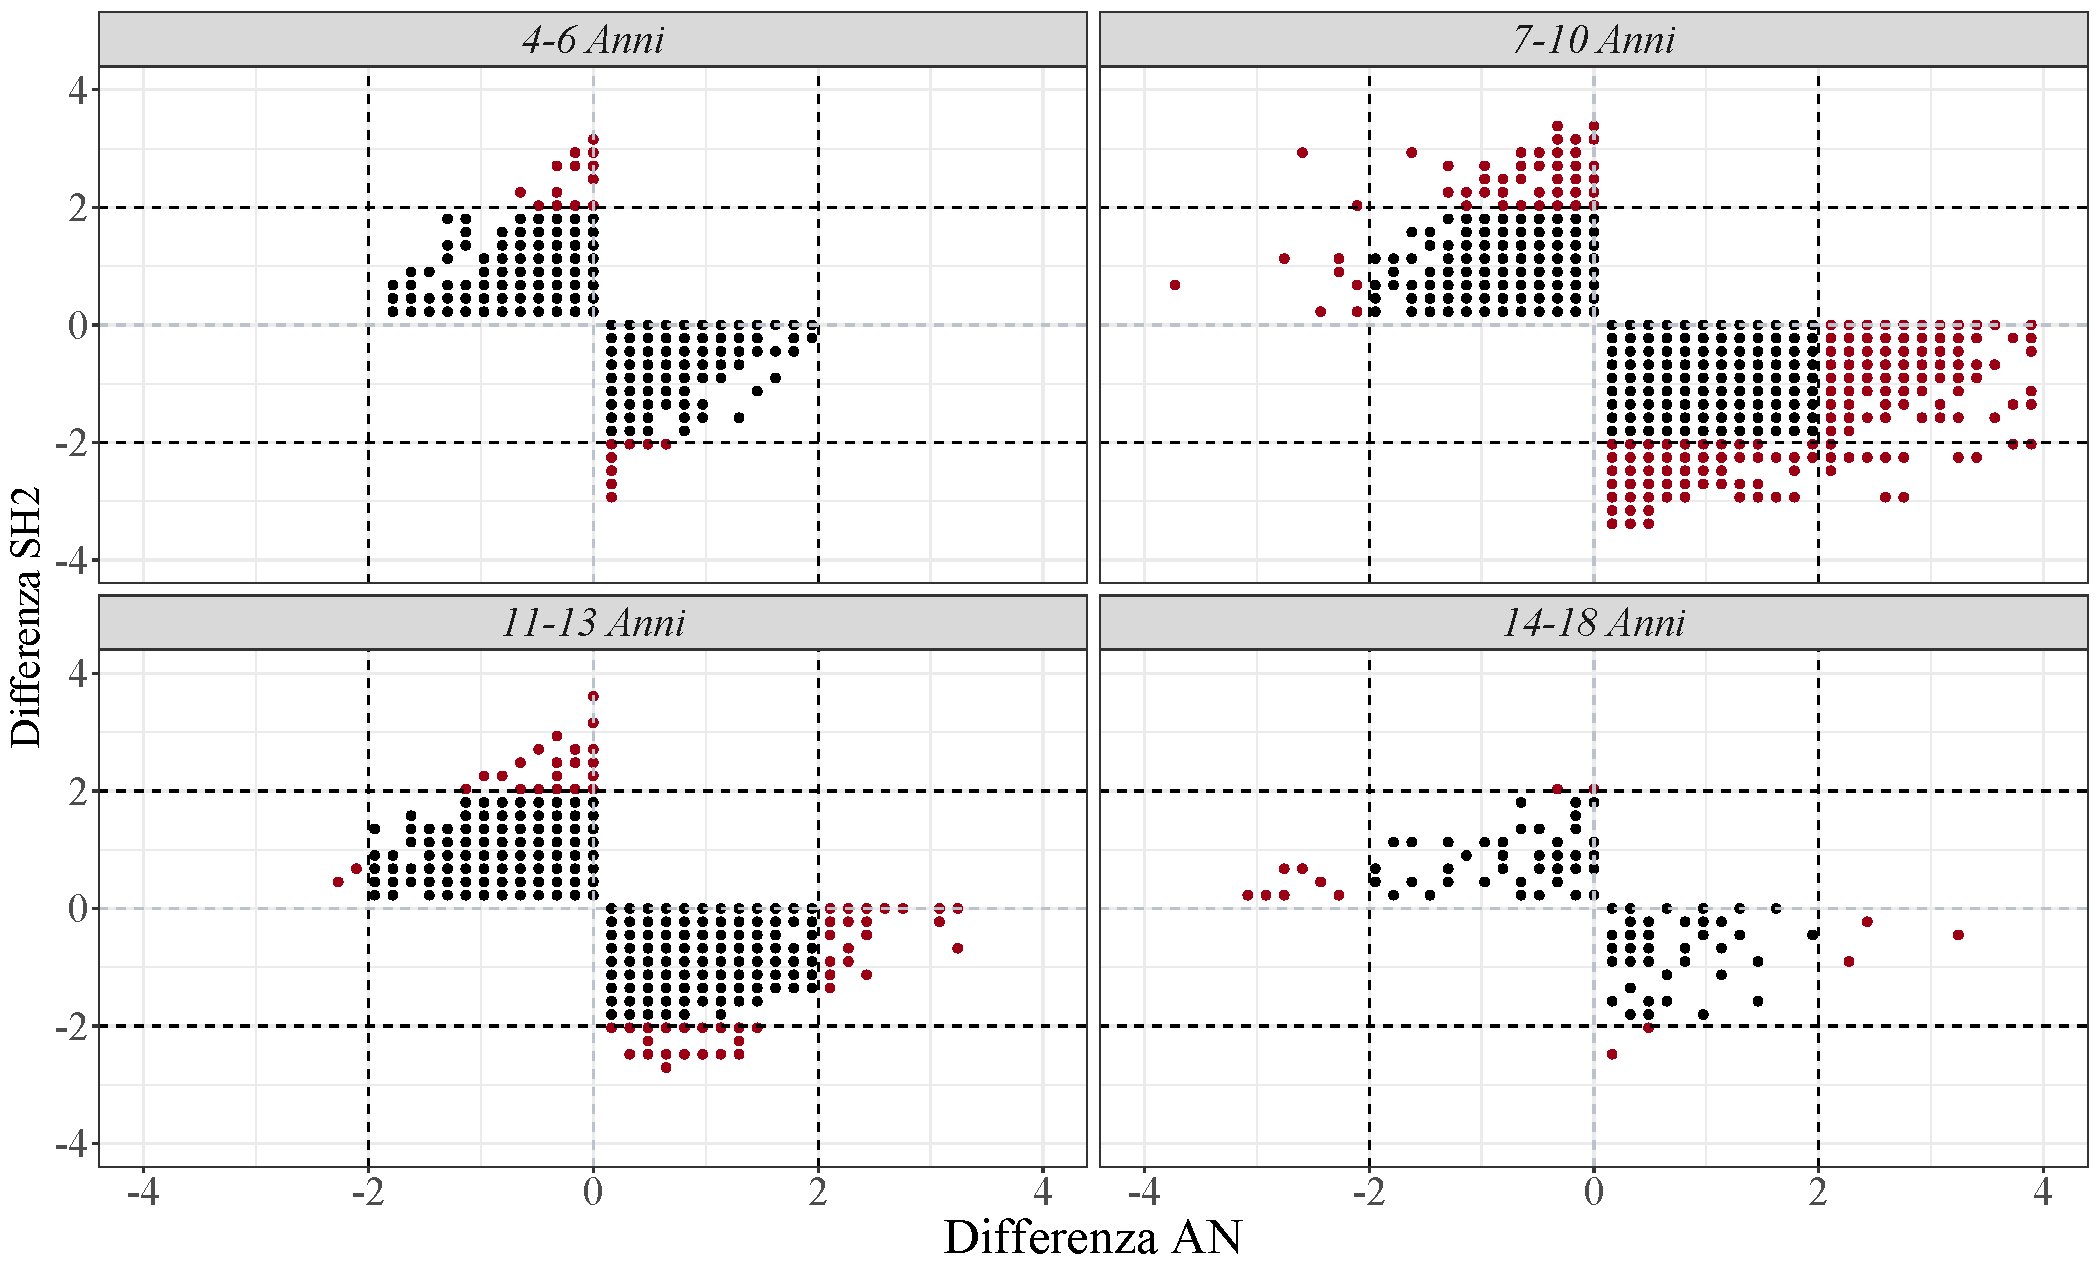
\includegraphics[width=\linewidth]{img/farfalle_gruppi_colored.pdf}

		
		
	\end{overprint}
\end{frame}

 
\end{document}